\hspace{3mm}

\centerline{\bf \Huge Домашнее задание}
\centerline{\bf \Huge Разнобой}

\begin{flushright}
    \scriptsize{Чтобы стать СИГМОЙ\\ нужно всего лишь решить это ДЗ на $13$ баллов}
\end{flushright}

\problem{1!} Расул Владимирович выписал на доску два числа. Михаил посчитал их НОД, и он оказался равен $2024$, а Лев посчитал НОК и получил такое же значение. Помогите Анджуру Аркадьевичу найти произведение двух чисел с доски.

\problem{2!} Найти НОК чисел $43560$ и $89100$ и объяснить свое решение, применив признаки делимости и ОТА!

\problem{3} В шиншиллах обучаются $26$ учеников среди них рыцари, которые всегда говорят правду, и лжецы, которые всегда лгут. Мог ли каждый сказать фразу: «Рыцарей нет среди всех шиншилл нет»?

\problem{4} Разрежьте фигуру на $4$ равные части по линиям сетки.

\begin{figure}[h]
        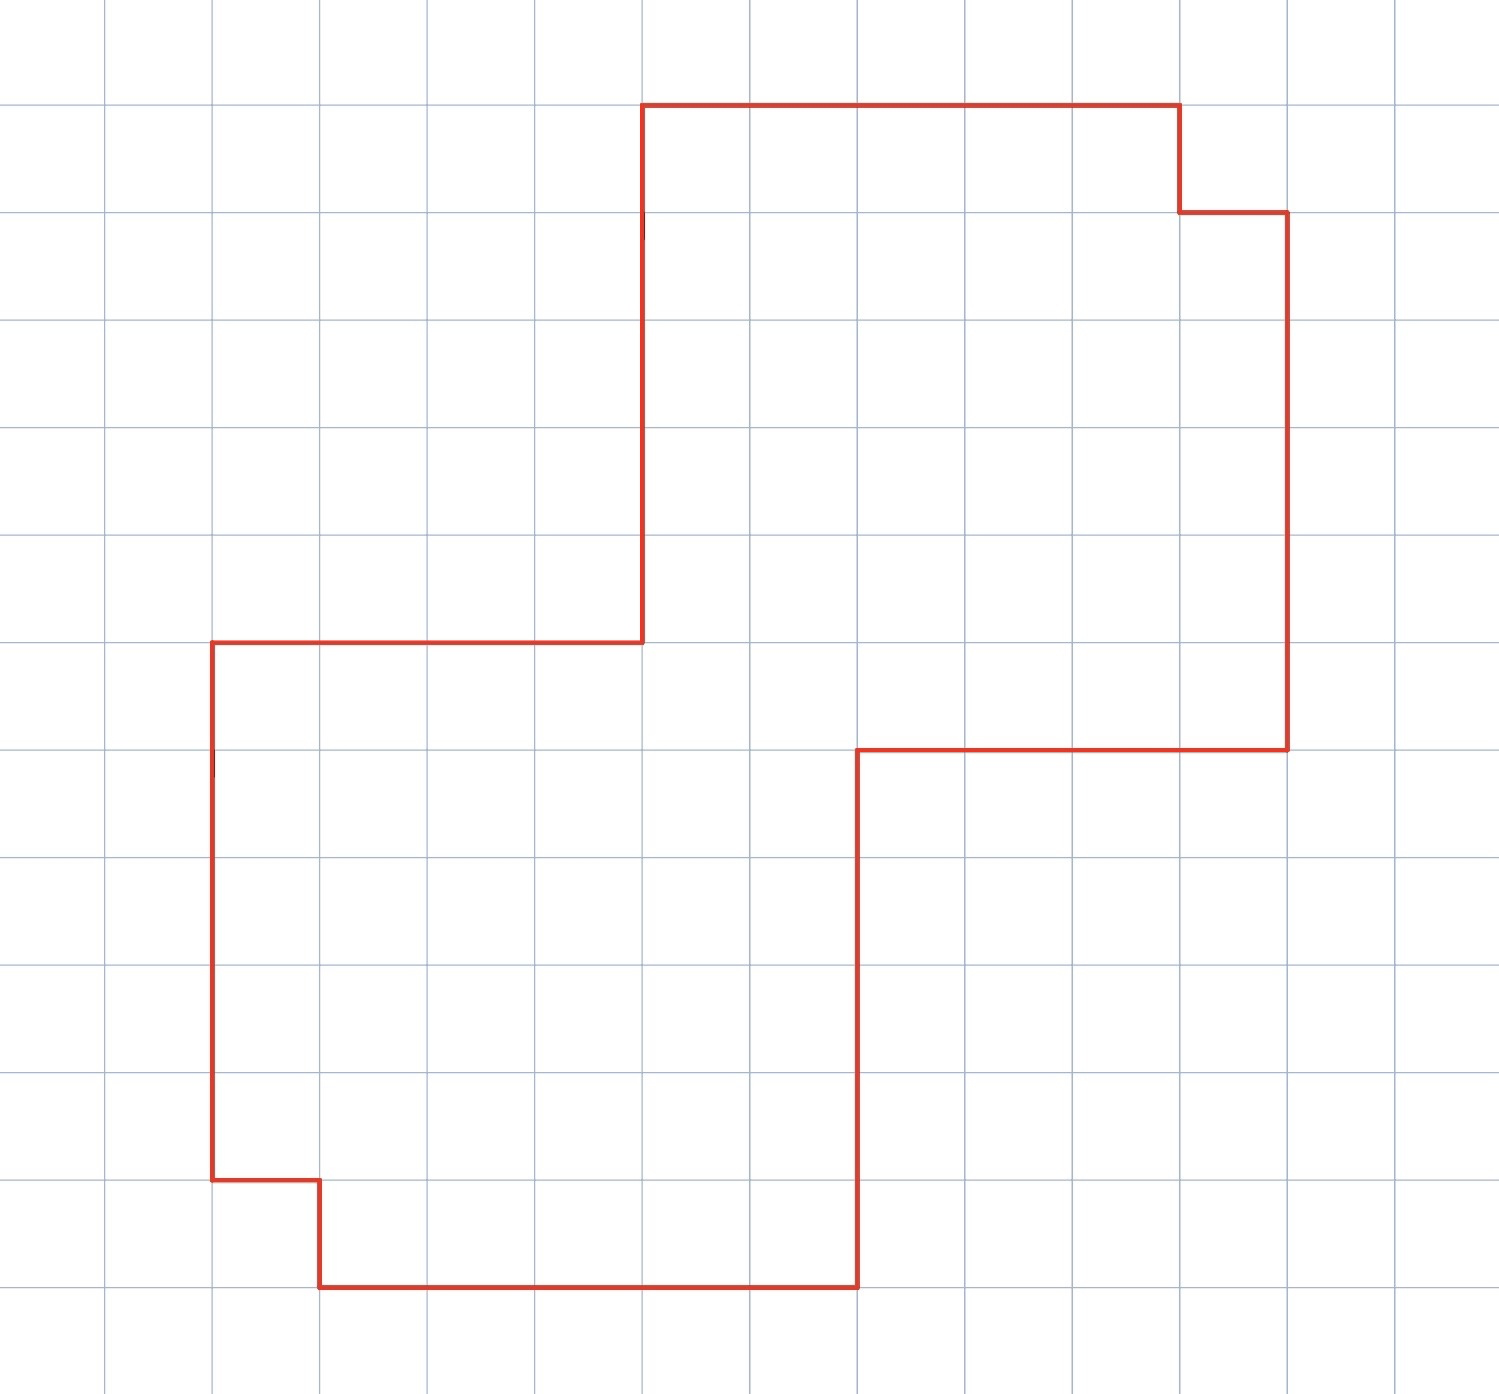
\includegraphics[width=0.5\linewidth]{ЭлМШ 2023-2024/VII блок/Шиншиллы/image.png}
\end{figure}